\subsection{PeerManager}\label{sec:mit-peerManager}
As the name suggests the \lstinline|PeerManager| is the component that takes care of \lstinline|RemotePeers|. Through the PeerManger other components can obtain all known RemotePeers, connect to new RemotPeers and destroy existing RemotePeers. Also messages are send via the PeerManager.

\paragraph{Obtaining RemotePeers} \label{paragraph:obtain-remotepeers}
Through at the PeerManager existing RemotePeers can be obtained. Existing RemotePeers are returned as a \lstinline|TableView| so the result can be filtered and sorted. The filter and sort operations do not affect the internal state of the peer manager because the TableView is exposed as a clone. 

By implementing the Observer pattern other components can subscribe on \textit{Peer-Churn}. \textit{Peer-Churn} means that subscribers are notified about \lstinline|Added| or \lstinline|Removed| peers so they can act accordingly.

\paragraph{Connect to a RemotePeer}
Through a given address the PeerManager can create a new RemotePeer and establish a connection. The connection can be either a direct connection which means a physical connection or a via connection. A via connection is opened for RemotePeers that are addressable by another direct RemotePeer. This happens when a client receives a message where the sender is not a direct peer.

\paragraph{Destroy a RemotePeer}
The PeerManager has the power to destroy a RemotePeer. In this process all connections to the RemotePeer are closed. 
Destroying a pear can either happen explicitly by calling the \lstinline|removePeer(remotePeer)| method or implicitly when the PeerManager notices that a RemotePeer does not have any open connections anymore.

Also it monitors direct connections that are bound to a via connection. When a direct connection is closed and there is no other open direct connection, the PeerManager also closes the via connection.

\begin{figure}[htb!]
  \centering
    \subfloat[]{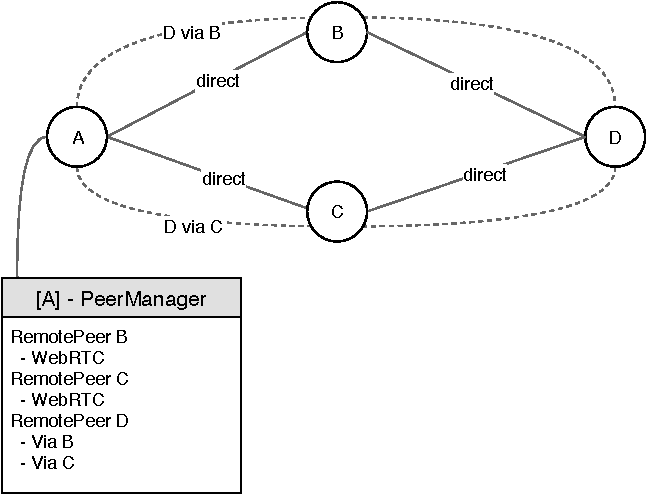
\includegraphics[width=0.4\textwidth]{graphics/implementation/mitosis-peer-manager.pdf} \label{fig:peer-manager-a}}
    \hspace{1 cm}
    \subfloat[]{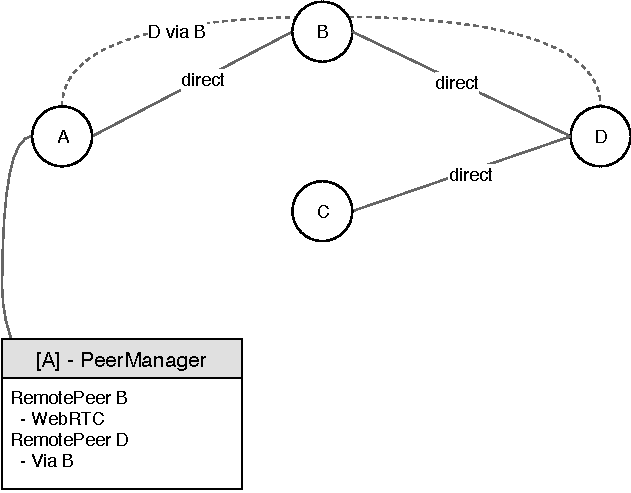
\includegraphics[width=0.4\textwidth]{graphics/implementation/mitosis-peer-manager-2.pdf} \label{fig:peer-manager-b}}
	\caption{PeerManager RemotePeer table}
\label{fig:peer-manager}
\end{figure}

\vref{fig:peer-manager} shows shows how the RemotePeer table of Mitosis Client \textit{A} would look like for the given connection state. \vref{fig:peer-manager-b} shows how the PeerManager is cleaning up RemotePeers and connections after loosing connection to Mitosis Client \textit{C}. 

\paragraph{Send a message}
Sending a message to a remote peer is also initiated via the PeerManager. As each peer has a quality, which is described in \vref{sec:peer-meter}, the PeerManager is selecting the peer with the best quality to transmit the message.